\documentclass{report}

\usepackage{listings}
\usepackage{fancyhdr}
\usepackage{graphicx}
\usepackage{amsmath}
\usepackage{ragged2e}
\graphicspath{{images/}}

\begin{document}
\begin{flushleft}
\large
\textbf{Instituto Tecnol\'ogico de Costa Rica, Sede Cartago}\\
\textbf{Escuela de Ingenier\'ia en Computaci\'on}\\
\textbf{Aseguramiento de la Calidad del Software}\\
\textbf{Proyecto Semestral I. Segmentaci\'on de c\'elulas} \\
\textbf{Profesor:} \\
M. Sc. Sa\'ul Calder\'on Ram\'irez \\
\textbf{Estudiantes:} \\                                                                                             
Jos\'e Enrique Alvarado Chaves, 201129079\\
Reggie Stewart Barker Guill\'en, 2014050578 \\
Joel Barrantes Garro, 2013120962 \\
Joel Schuster Valverde, 2014096796 \\
\textbf{6 de marzo del 2017} \\

\end{flushleft}

\begin{center}
\huge  \textbf{Prueba de concepto}
\end{center}
\large
\begin{center}
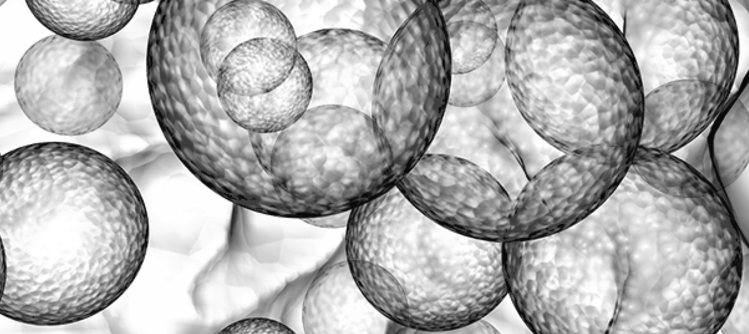
\includegraphics [scale = 0.70]{celulas.png}\\ [0.5 cm] 
\end{center}
El presente documento es parte de la prueba de concepto del primer proyecto del curso de ``Aseguramiento de software", en el cual se pretende realizar un conjunto de investigaciones que permitir\'an ver la factibilidad de las ideas, tecnolog\'ias o funciones investigadas por el grupo de trabajo. \\ 

Ahora bien, para la lectura del documento se presentar\'a primero un conjunto de experiencias las cuales orientaron y conllevaron al equipo escoger las tecnolog\'ias-herramientas. Luego una estructura de alto nivel del problema y las principales subpartes de la primera parte del proyecto. Al final se presentan algunos de los problemas que se tuvieron en los algoritmos sobre las im\'agenes.\\ [3 cm]

\huge  Experiencia:\\

\large 
El primer acercamiento del grupo fue para tener una definici\'on acerca de las herramientas para el uso de: \\

\begin{itemize}
\item Repositorio de versiones 
\item Versi\'on de OpenCV 
\item Versi\'on de java. 
\item Versi\'on de IDE.
\end{itemize}
 
Para la selecci\'on del repositorio de versiones se seleccion\'o github al inicio por convenci\'on del equipo, debido a su experiencia en este. Por otra lado en la selecci\'on de la versi\'on de OpenCV se acord\'o utilizar la versi\'on con m\'as documentaci\'on para una mayor facilidad a la hora del desarrollo del proyecto, la documentaci\'on de OpenCV conllevo a seleccionar java 1.7 debido a que se presenta la recomendaci\'on utilizar dicha versi\'on para una mayor estabilidad en el sistema.  
Para la selecci\'on del IDE se present\'o la utilizaci\'on de Eclipse Indigo, siendo este una de las versiones viejas de la plataforma, pero al mismo tiempo una de las que posee una interfaz de usuario m\'as estable y veloz. \\

Para el segundo acercamiento se presentaron algunas propuestas y se cambiaron algunas de las herramientas presentadas.  \\

\textbf{Cambios realizados:}
\begin{itemize}  
\item Versi\'on de java. 
\item Versi\'on de OpenCV. 
\item Versi\'on de IDE. \\
\end{itemize}

\textbf{Propuestas realizadas:}
\begin{itemize} 
\item Utilizar Angular 2 para el desarrollo del cliente. 
\item Utilizar Tomcat Native para crear el lado de servidor. 
\item Utilizar Spring para crear el lado de servidor. 
\item Utilizar Jersey para crear el lado de servidor. \\
\end{itemize}

Los cambios realizados sobre la versi\'on de java se debieron a que las actualizaciones sobre la versi\'on de OpenCV facilita varias funciones sobre el proyecto a desempeñar, pero como consecuente se pide una actualizaci\'on de la versi\'on de java utilizada a la versi\'on 1.8. Al mismo tiempo que tres integrantes se encargaban del \'area de openCV y ve\'ian esta dificultad, tambi\'en se encontraba el compañero restante que se encarg\'o del lado del servidor, en el cual encontraba m\'as facilidad el usar java 1.8 debido a las caracter\'isticas que se prove\'ian en las versiones actualizadas de las herramientas de Spring y Jersey. Al cambiar a la versi\'on de java 8, se cambio adem\'as el IDE de la versi\'on Indigo por Neon, debido a que posee mas facilidades a nivel de interfaz de usuario, pero se sacrifica rendimiento.\\

Algunas otras herramientas probadas fueron Jersey y Tomcat, que permiten la realizaci\'on de servicios web con java, pero el equipo ha optado por el uso de la herramienta Spring para la construcci\'on de un servicio web RESTful. Las principales razones para la utilizaci\'on de la misma, es la facilidad del manejo de dependencias que tienen Spring-maven, uso de patrones de dise\~no que proporcionan varias facilidades como por ejemplo la instanciaci\'on de objetos en java y por \'ultimo la facilidad de comunicar la misma con diferentes tecnolog\'ias ya sean de bases de datos o otros servicios. \\

Por \'ultimo, una de las \'areas que se empez\'o a investigar por parte de dos de los miembros fue el uso de angular 2, para el desarrollo del lado del servidor, que proporciona facilidades como el manejo de dependencias del lado del cliente y adem\'as un conjunto de importante de caracter\'isticas que lo hacen amigable al usuario. Por problemas con respecto al aumento en la curva de aprendizaje en esta otra herramienta se decide utilizar Spring MVC temporalmente para proporcionar al cliente una interfaz que permita interactuar de forma amigable. \\

Como resultado a esta primera etapa del proyecto se estructura el sistema con las siguientes herramientas: 
\begin{itemize}
\item Spring MVC 4.0. 
\item Spring GS – Uploading files 0.1.0. 
\item Maven 4.0.0. 
\item OpenCV 3.2.0. 
\end{itemize}

Para los pr\'oximos entregables se ver\'a la utilizaci\'on formal de Spring JPA y hibernate. \\
Enlace a proyecto en repositorio Git:  https://github.com/schust3r/PSA \\ [0.5 cm]

\huge  Estructura de alto nivel del sistema.\\

\LARGE 
Diagrama de componentes \\[0.5 cm]

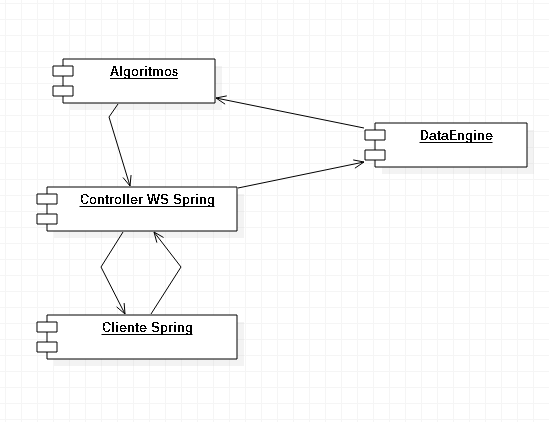
\includegraphics [scale = 1]{Diagrama.png}\\ [0.5 cm] 

\LARGE An\'alisis b\'asico de los trozos\\
\large
\begin{flushleft} 
 \textbf{1) C\'alculo de umbral \'optimo utilizando el algoritmo de Kittler}\\[0.1 cm]%----------------------------------------------------------
Implementaci\'on del algoritmo de Kittler determinar un valor \'optimo con el fin de umbralizar una imagen.\\[0.1 cm]

\textbf{Entrada(s):}\\
Tipo: Mat\\
Matriz de p\'ixeles correspondientes a una imagen en escala de grises.\\
\textbf{Salida(s):}\\
	Tipo: Int\\
\textbf{Umbral \'optimo} \\
	 \(\tau\) \(\in\) \{0,1,2,...,254,255\}\\[0.5 cm]

\textbf{2) Umbralizaci\'on de la imagen usando un valor arbitrario.}\\%----------------------------------------------------------
Toma como entrada una matriz de p\'ixeles de una imagen en escala de grises para producir una matriz binaria con entradas aij, con \hspace{1cm}aij =0 o aij = 255.

\textbf{Entrada(s):}\\
 Tipo: Mat\\
Matriz de p\'ixeles correspondientes a una imagen en escala de grises.

Tipo: Int\\
\textbf{Umbral \'optimo} \\
	 \(\tau\) \(\in\) \{0,1,2,...,254,255\}\\[0.3 cm]

\textbf{Salida(s):}\\
Tipo: Mat\\
Matriz de p\'ixeles correspondiente a una imagen umbralizada con entradas aij, con aij =0 o aij = 255.\\[0.5 cm]

\textbf{3) Etiquetado de una imagen umbralizada}%----------------------------------------------------------
Genera una nueva matriz representando el etiquetado de una matriz umbralizada.\\[0.1 cm]

\textbf{Entrada(s):}\\[0.1 cm]
	Matriz de p\'ixeles correspondiente a una imagen umbralizada con entradas aij, con aij =0 o aij = 255\\
\textbf{Salida(s):}\\[0.1 cm]
	Tipo: Mat\\
	Matriz con p\'ixeles en el rango de colores RGB .\\[0.5 cm]

\textbf{4) Carga de imagen}%----------------------------------------------------------
Permitir al usuario subir una imagen desde el cliente y guardarla en el servicio web. \\[0.3 cm]


\textbf{Lado del cliente:} \\[0.1 cm]
\textbf{Entrada(s):} \\
	Imagen prove\'ida por el usuario final.  \\
\textbf{Salida(s):} \\
	Imagen enviada a trav\'es del protocolo de transferencia de hipertexto, prove\'ido por la herramienta de spring. \\[0.3 cm]
 
\textbf{Lado del servidor:} \\[0.1 cm]
\textbf{Entrada(s): }\\
	Imagen recibida por el lado del cliente con http, en Spring MVC. \\
 
\textbf{Salida(s): }\\
	Imagen se guarda en el lado del servidor. \\[0.5 cm]
\end{flushleft} 

\large 
\huge Repaso de la experiencia y algunos problemas encontrados en algoritmos-funciones. \\ [ 0.2 cm]

\large Uno de los principales problemas encontrados durante el proyecto fue el manejo de versiones de las herramientas que se ten\'ia en proceso de investigaci\'on, para posteriormente  implementar en el proyecto. Por otro lado, en la investigaci\'on se tuvieron algunos problemas sobre las funciones de las herramientas escogidas, puesto que la documentaci\'on variaba considerablemente con respecto a las versiones.\\ [0.3 cm]
Para finalizar no se tuvieron problemas a la hora de la utilizaci\'on de los algoritmos de la herramienta OpenCV, puesto que una vez que el equipo logr\'o hacer la instalaci\'on formal de todas las herramientas para el desarrollo, se invirti\'o tiempo en la lectura de entradas-salidas de los algoritmos necesarios para completar la primera etapa del POC.

\end{document}
